
%%%%%%%%%%%%%%%%%%%%%%%%%%%%%%%%%%%%%%%%
%%%%%%%%%%%%%%%%%%%%%%%%%%%%%%%%%%%%%%%%
\section{Introduction}
%%%%%%%%%%%%%%%%%%%%%%%%%%%%%%%%%%%%%%%%
%%%%%%%%%%%%%%%%%%%%%%%%%%%%%%%%%%%%%%%%

%%% Intro & CO/GC description:
Recombination is a fundamental component of meiotic cell division, and the reshuffling of genetic variation has important evolutionary implications, enabling the action of natural selection.
DNA double strand breaks (DSBs) resolve to one of two possible outcomes: crossover (CO) and non-crossover, or gene conversion (GC).
Most research to date has been focused on the large-scale chromosomal exchanges that accompany CO, which are easily detected with a variety of direct and indirect methods.
In contrast, gene conversion (GC), is a non-reciprocal process in which short segments of DNA are transferred from one parental chromosome to another.

Molecular studies support a model in which DNA DSBs occur at multiple points along a chromosome, and each of these DSBs undergoes a repair procedure that results in either CO or GC\cite{Baudat2007}.
Sperm typing studies have estimated that GC occurs approximately ten times more frequently than crossover\cite{Jeffreys2004,Baudat2007,Cole2012}.
Gene conversion events are small, typically under 1000 bp, but could range from 50-2000 bp\cite{Jeffreys2004}.
This small size therefore makes GC events difficult to detect using genome-wide inference methods such as pedigree studies or even linkage disequilibrium (LD) analysis.

Despite these difficulties, gene conversion has been successfully studied using pedigree approaches.
A recent study used SNP array data from multiple three-generation pedigrees to identify approximately 100 GC events in humans\cite{Williams2015}. 
Supporting results from molecular studies, gene conversions were found to occupy 100-1000 bp tracts.
However, GC events were found to cluster unexpectedly, raising questions as to potential differences in the repair mechanism.

% biased gene conversion
Gene conversion has been also shown to be biased in the exchange of alleles\cite{Chen2007}.
When occurring around a heterozygous SNP, GC can result in the non-Mendelian transfer of alleles, with the donor allele copied in a 3:1 ratio over the allele on the recipient chromosome.
Furthermore, the copied allele is not chosen completely at random, and there is a dependency in which certain alleles are favored over others.
Weak alleles (A and T) tend to be replaced with strong alleles (G and C). % Duret et al., 2006; Duret and Galtier, 2009; Webster and Hurst, 2012)
This is known as GC biased gene conversion (gcBGC), the over-transmission of G and C alleles during recombination.
Biased gene conversion has evolutionary implications, and has contributed to an ongoing change on the base content of the genome\cite{Bherer2014}.

Several statistical approaches have been proposed to create a model with which to detect gene conversion events from population genetic data.
\citet{Gay2007} created a hidden Markov model (HMM) that models gene conversion together with crossover.
This model was based upon a previous method for detecting recombination using patterns of LD, which modeled haplotype segments as a copied mosaic of previously observed haplotypes\cite{Li2003}.
Another model, although it does not explicitly model gene conversion, is HAPMIX\cite{Price2009}, which adapts the Li and Stephens model to perform ancestry deconvolution on admixed genomes.
In this model, two divergent populations of haplotypes serve as a reference, and the admixed haplotype can copy from either population, with cross-population switches reflecting a change in haplotype ancestry.
HAPMIX has been demonstrated to have a high sensitivity for partitioning admixed genomes\cite{Price2009}.

The HAPMIX approach highlights a relatively new method of studying recombination in human populations having recent admixture.
In this method, an admixed genome is modeled as a mosaic of haplotypes from two ancestral reference populations that have divergent patterns of allele frequencies (Figure \ref{fig:GCadmixture}).
This technique was recently used to study recombination in African American populations\cite{Hinch2011}.
This study found further evidence of population-specific hotspots, finding 2,500 hotspots unique to West Africans, and finding that these are tied to a novel PRDM9 binding motif.


\afterpage{
\begin{figure}[P]
    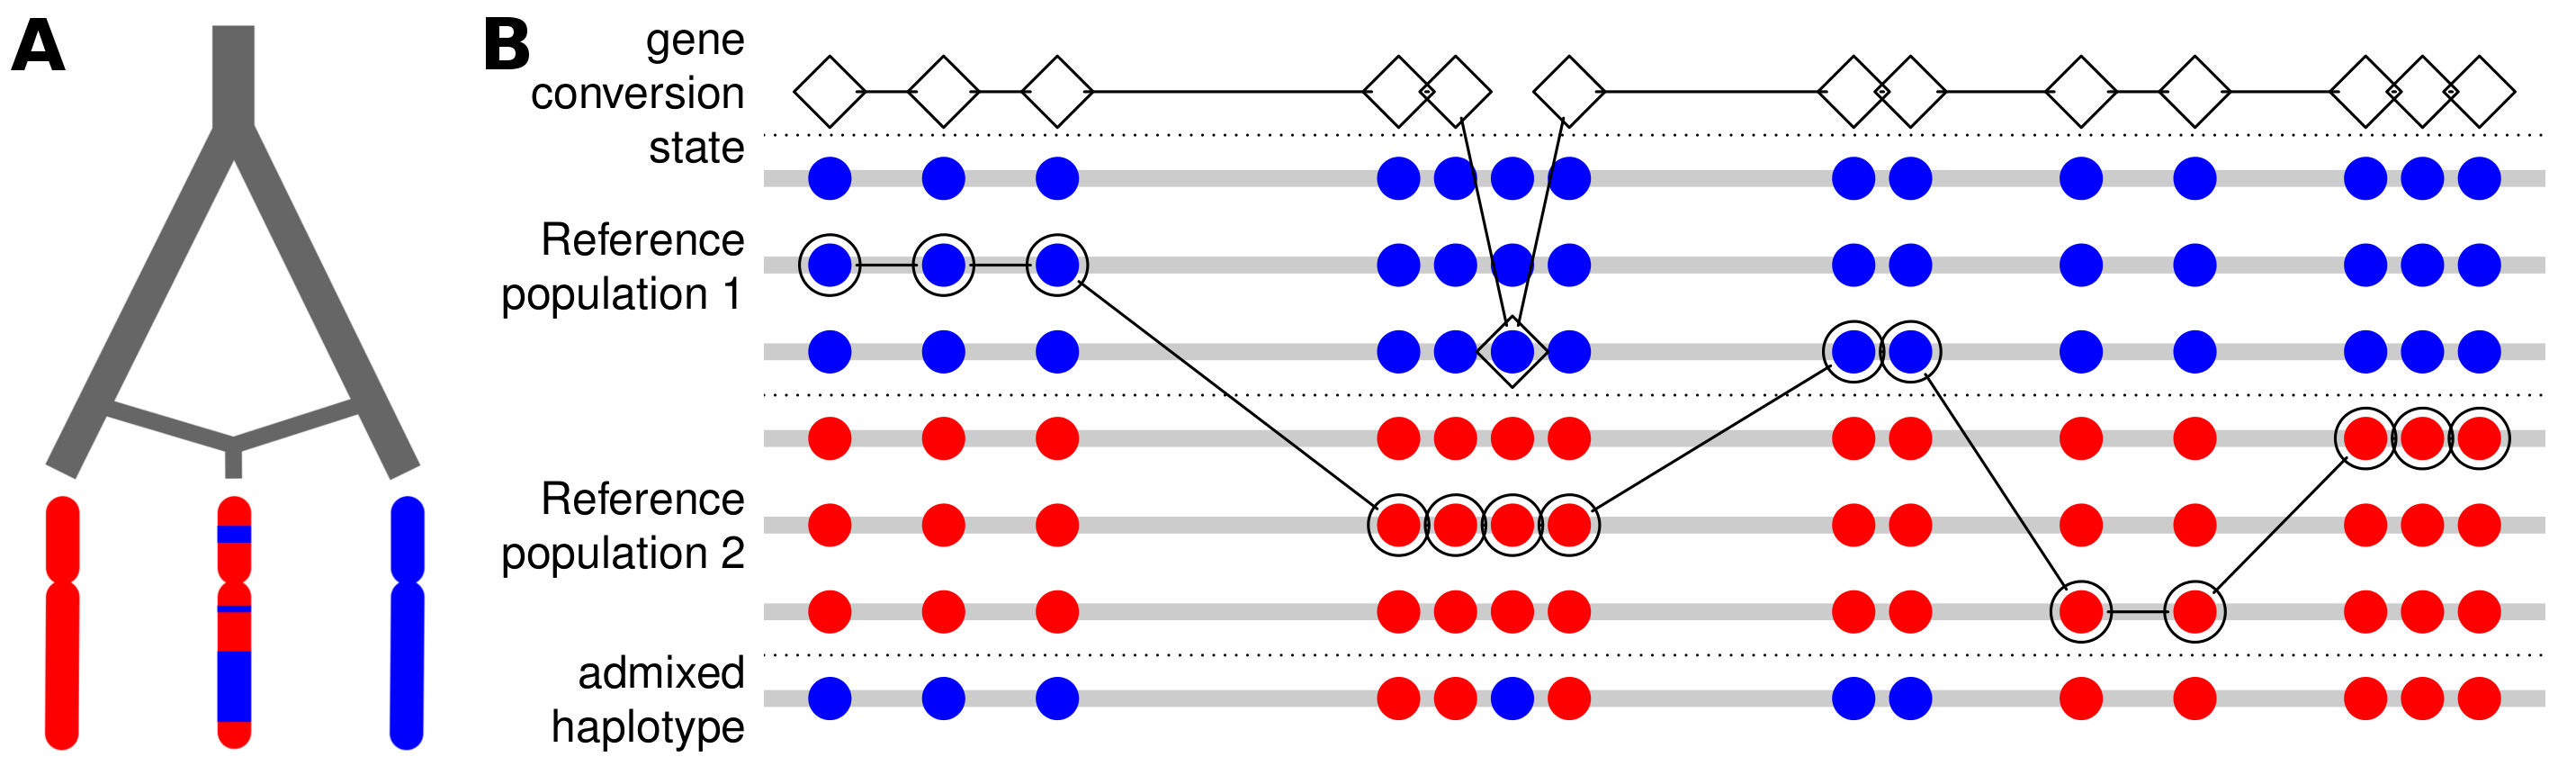
\includegraphics[width=\textwidth]{geneConv/figs/admix_HMM.png} \vspace{-10pt}
    \captionTitle{\textbf{Admixture approach to gene conversion detection.}}{
        (\textbf{A}) An admixed genome is shown (center) as a mixture of genomic segments from two divergent ancestral populations.
        (\textbf{B}) Diagram showing haplotypes in our HMM.
        Each horizontal line is a haplotype and each column of circles represents the alleles of a SNP, with blue and red colors designating alleles that are representative of two divergent ancestral reference populations.
        The haplotypes for the reference populations are used as templates for the admixed haplotype (bottom). %, in which the alleles are of unknown ancestry.
        The state path of haplotype transitions ($X$) is shown by open circles.
        The gene conversion state path ($G$) is shown in open diamonds.
        In this example there is one gene conversion event at SNP 6 in the admixed haplotype, which is copied from a haplotype in population 1.
        In all other SNPs there is no gene conversion ($G=0$).
        \label{fig:GCadmixture} } 
\end{figure}
\clearpage}
%%%

Here, we will combine key features from each of these two models to develop a new method to detect gene conversion.
Our method aims to detect gene conversion events using admixed population genetic data, where a gene conversion from on population will be detectable with increased contrast against the background of the other divergent population.
From HAPMIX, we use the convention of modeling recombination separately both prior to, and after a point admixture event.
From the \citet{Gay2007} model, we model crossover and gene conversion with independent Markov chains.
Using a combination of these two methods, our model provides a novel method to detect gene conversion events in humans using admixed genomes.


%%%%%%%%%%%%%%%%%%%%%%%%%%%%%%%%%%%%%%%%
%%%%%%%%%%%%%%%%%%%%%%%%%%%%%%%%%%%%%%%%
\section{Methods}
%%%%%%%%%%%%%%%%%%%%%%%%%%%%%%%%%%%%%%%%
%%%%%%%%%%%%%%%%%%%%%%%%%%%%%%%%%%%%%%%%

% $ \Pr( h_{j+1} | h_1, \ldots, k_j, \rho, \gamma ) $

We provide here details of the implementation on the hidden Markov model used.
We build upon the hidden Markov model framework put forth by \citet{Li2003}, in which an unknown haplotype is modeled as an imperfect mosaic of previously observed haplotypes.
We adopt features from several extensions of this framework that have been used to address population genetics problems in recent years.
The HAPMIX model\cite{Price2009} has been used successfully in the deconvolution of admixed genomes.
In HAPMIX, the Li and Stephens model is modified to include two separate groups of reference populations, corresponding to ancestral populations, from which segments of an unknown admixed haplotype can be assigned.
The Li and Stephens model has also been modified for the detection of gene conversion events, which can be achieved by modeling gene conversion and crossover events simultaneously\citep{Gay2007}.

Here, we take key elements from each of these models: from HAPMIX the use of two divergent reference populations to increase contrast in ancestry, and from the \citet{Gay2007} model the addition of a second Markov chain to model gene conversion events.
Using the ancestry deconvolution approach we can assign blocks of sequence to one ancestral population or the other.
In a block of sequence assigned to one ancestral population, gene conversion events from the other population will stand out against this background, and enable more accurate identification of these events.

\subsection{Model details}
We model gene conversion events along with haplotype transitions (crossovers) as independent Markov processes with transitions possible between each.
In our model an admixed haplotype is composed of an imperfect mosaic of haplotypes from two ancestral populations, labeled $P_1$ and $P_2$, containing $n_1$ and $n_2$ haplotypes, respectively.
We assume that the unknown, admixed haplotype underwent a point admixture event $T$ generations in the past,
in which a proportion, $\mu_1$, of that haplotype's ancestry comes from $P_1$, with the remainder, $\mu_2 = 1-\mu_1$, contributed from $P_2$.

The crossover chain is affected by both ancient and recent crossover events.
Ancient events are controlled by the population crossover rate, $\rho = 4 N_e r$, where $N_e$ is the effective population size and $r$ is the per-generation recombination rate.
From HAPMIX, recent recombination events are modeled by considering the per generation recombination rate, $r$, and the estimated time since the admixture event, $T$.
This $T$ parameter allows the per generation recombination rate to be scaled to account only for recent events, and model specifically switches in ancestry.
The $\rho$ parameter is allowed to vary across regions tested in our model, and we use a genetic map to obtain the recombination rate $r$.

From the \citet{Gay2007} model, the gene conversion chain is modeled similarly, with the frequency of gene conversion affected by the population gene conversion rate $\gamma = 4 N_e g$, where $g$ is the per-generation gene conversion rate.
%However, we we do not attempt to capture events that occurred previous to the admixture event, and we thus omit the population scaled gene conversion rate,
We the HAPMIX convention of modeling recent events using the per-generation gene conversion rate, $g$ and the time since admixture, $T$.
At the same time, we model ancient gene conversion events, prior to admixture, using the $\gamma$ parameter.

% our HMM consists of terms, $\Pr(h_1,\ldots,h_{(n_1+n_2)},\rho_1,\rho_2,\gamma_1,\gamma_2)$.
% Our HMM has $(n_1+n_2)+(n_1+n_2)^2$ possible states, where $X_j$ represents the parental haplotype copied at site $j$ and $G_j$ represents the gene conversion state at site $j$.

\paragraph*{Parameter settings.}
We use two divergent reference populations, arbitrarily labeled.
The first, population $P_1$, will be used to represent Europeans, while the second, $P_2$, will represent a population of African origin.
We take into account the differences in effective population size, $N_e$, by setting $N_{e1} = 10,000$ and $N_{e2} = 18,000$.
The population sizes translate to differences in the population recombination and gene conversion parameters for each population, giving $\rho_1$, $\rho_2$, $\gamma_1$, and $\gamma_2$.
We use the HapMap genetic map\cite{hapmap2007} to obtain the recombination rate between pairs of sites.
We set $T$ to be 7 generations, and assume the ancestry contribution from Europeans, $\mu_1$, is 0.2.
We set the ratio between gene conversion and crossover rate, $f = g / r = 10$, based on estimates previously made using sperm typing\cite{Jeffreys2004} and population genetic\cite{Gay2007} data.
The expected length of a gene conversion tract, $1/\lambda$, is fixed at 500bp.

\subsection{Transition probabilities}
Following \citet{Gay2007}, the transition probabilities for crossover ($X$) and gene conversion ($G$) chains occur simultaneously.
The crossover chain is independent and depends only upon the previous state within its own chain.
However, it was necessary to consider gene conversion in the context of the current population of the crossover chain because our approach relies on the detection of gene conversion events that are copied from a different population from the haplotype as a whole.
Therefore, we make a modification to the transition probabilities of the gene conversion chain:
%
\begin{equation} \Pr(X_{j+1}, G_{j+1} | X_{j},G_{j} ) = \Pr(X_{j+1}|X_{j}) \Pr(G_{j+1}|G_{j},X_{j}) ~. \end{equation}

For each site we consider the transition from one haplotype to another, taking into account population specific parameters for $\rho$, $\gamma$, $\mu$, and $n$.
If the destination haplotype belongs to $P_1$ we use $\rho_1$, $\gamma_1$, $\mu_1$ and $n_1$; for haplotypes transitioning into $P_2$, $\rho_2$, $\gamma_2$, $\mu_2 = 1-\mu_1$, and $n_2$.
%We consider the possibility of switching between the two parental populations, and we label the source (previous) population $p_k$ and the destination population (at site $j+1$) $p_l$.
The population containing the haplotype at site $j$ is labeled $p_k$, and the population that contains the destination haplotype, at site $j+1$, is labeled $p_l$.


\subsubsection*{Starting probabilities}
%%%
% The probability of the crossover chain starting in any given haplotype is scaled by the estimated ancestry contribution ($\mu$) from each population to the admixed haplotype:
There is an equal probability of starting the crossover chain in any given haplotype, scaled by the estimated ancestry contribution ($\mu$) from each population to the admixed haplotype, where $x \in p_l$:
\begin{equation} \Pr(X_1 = x) = 
        \mu_l/n_l ~.
%\begin{dcases}
%        %\mu_1/n_1 & \text{if $x \in p_1$} \\
%        %(1-\mu_1) /n_2 & \text{if $x \in p_2$} ~.
%\end{dcases}
\end{equation}
%%%
The gene conversion chain can start either within or outside of a gene conversion state.
For the null state we consider the possibility of having ended a gene conversion tract from any of the haplotypes, and the estimated rate of gene conversion since admixture.
The gene conversion chain can also start within a haplotype in each of our two reference populations, dependent on the expected rate of gene conversion since admixture and weighting the haplotypes of each population by the ancestry contribution, $\mu$, to the admixed haplotype.
%The parameter $\mu$ is used to weight the number of haplotypes by their expected ancestry contribution to the admixed haplotype.
Since we have no information outside this first site, we set the value of $g = f r$, where we use the estimated genome-wide recombination rate of 1.1 cM/Mb for $r$.
\begin{equation} 
\Pr(G_1 = g) =  \\
\begin{dcases}
    \frac{\lambda (n_1+n_2) }{ \lambda (n_1+n_2) + g T }
& \text{if $g = 0$} \\
    \frac{ g  T }{ \lambda (n_1+n_2) + g T } \frac{\mu_l}{n_l}
& \text{if $g \ne 0$ and $g \in p_l$} \\
\end{dcases}
\end{equation}


%%%%%%%%%%%%%%%%%%%%%%%%%%%%%%%%%%%%%%%%%%%%%%%%%%
%%%%%%%%%%% X transitions
%%%%%%%%%%%%%%%%%%%%%%%%%%%%%%%%%%%%%%%%%%%%%%%%%%

\subsubsection*{Crossover transition probabilities}
The probability of transitioning from a hidden state at site $j$ to a hidden state at site $j+1$ depends on several parameters,
including the physical distance $d_j$ (in base pairs) and recombination rate, $r_j$ (e.g., cM/Mb).
We adopt the approach used by HAPMIX to capture recent crossovers since admixture as a product of the per-generation genetic distance between markers, $r_j d_j$, and the number of generations since admixture, $T$.
Ancient recombination is modeled using the population scaled recombination rate, $\rho$, scaled by the number of haplotypes in the population.
Each population has its own $\rho$ parameter, which depends on the effective population size.
%
\begin{multline}
     \Pr(X_{j+1}=x' | X_{j}=x) = \\
\begin{cases}
%\displaystyle 
\hfill   (1-e^{-r_j d_j T}) \frac{\mu_l}{n_l}  
        &  \text{if $x \ne x'$ and $p_k \ne p_l$ } \\
%\displaystyle     
\hfill e^{-r_j d_j T} (1-e^{-\rho_{l,j} d_j / n_l }) \frac{1}{n_l} + 
        (1-e^{-r_j d_j T}) \frac{\mu_l}{n_l}  
        &  \text{if $x \ne x'$ and $p_k = p_l$ } \\
%\displaystyle 
        e^{-r_j d_j T} e^{-\rho_{l,j} d_j / n_l } +
        e^{-r_j d_j T} (1-e^{-\rho_{l,j} d_j / n_l }) \frac{1}{n_l} + 
        (1-e^{-r_j d_j T}) \frac{\mu_l}{n_l}
        &  \text{if $x=x'$ and $p_k = p_l$ } \\
        %
\end{cases}
\end{multline}

%%%%%%%%%%%%%%%%%%%%%%%%%%%%%%%%%%%%%%%%%%%%%%%%%%
%%%%%%%%%%% G transitions
%%%%%%%%%%%%%%%%%%%%%%%%%%%%%%%%%%%%%%%%%%%%%%%%%%

\subsubsection*{Gene conversion transition probabilities}
Here we follow the \citet{Gay2007} model with modifications to account for the two ancestral populations and switches between them, focusing on identifying the recent events since admixture.
In the case where $X_j$ and $G_j$ occur within the same population, we must account for gene conversions occurring both prior to, and since the admixture event.
The population scaled rate, $\gamma$, is used to model gene conversion events occurring prior to admixture.
For gene conversions occurring after the admixture event, we use the HAPMIX convention, as in the crossover transitions, of modeling recent gene conversion events by the per generation gene conversion rate, $g$, and the number of generations since admixture, $T$.
We are specifically interested in capturing the situation in which $X_j$ and $G_j$ occur across different populations.
In this case, we do not model ancient events, but focus on capturing only recent gene conversions.

Generally, the probability of both starting a gene conversion and ending one within the interval is taken into account to determine $\Pr(G_{j+1}|G_j,X_j)$.
The rate of ending a gene conversion tract, $\lambda$, is modeled geometrically as a function of physical distance.
This allows allowing termination to occur at any point within the interval and for the tract to ``reset'' at any time regardless of the current state. %%% fix this
The probability of starting a gene conversion event is given by the product of $g$ and the number of generations since admixture, $T$.
%We expand the \citet{Gay2007} model to include two independent $\gamma$ parameters, one for each population.



\paragraph{The gene conversion null state.}
In the first transition, we move from a null gene conversion state ($G_j=0$) to another null gene conversion state ($G_{j+1}=0$).
This is given by the probability of having no reset event and no gene conversion event in the interval, either prior to, or after admixture.
%
\begin{equation} \label{eq:Gnull}
    \begin{split}
        \Pr(G_{j+1}=0|G_{j}=0,X_j=x) = \\
        e^{-\lambda d_j} e^{-g_j d_j T } e^{-d_j \gamma_l/n_l} +
    \int_0^{d_j} \lambda e^{-\lambda x} e^{-g_j x T } e^{-x \gamma_l/n_l } ~\mathrm{d}x ~~~
     \text{if $x \in p_l $ } \\%[1em]
\end{split}
\end{equation}
%
The integral represents the possibility that there was a reset event, but no gene conversion event.

\paragraph{Entering a gene conversion event.}
The second transition describes the probability of entering a gene conversion state from a null state.
When $g$ and $x$ are within the same population, we must account for gene conversions events occurring prior to admixture, as well as those occurring after.
We use the following constant, $Z$, to scale the gene conversion rate.
The left term accounts for the post-admixture gene conversion rate, $g_j T$, scaled by $u_l/n_l$ for the target population.
The right term captures events occurring prior to admixture, using the population scaled gene conversion rate $\gamma_l/n_l$.
\newcommand{\constZ}{\bigg[ \frac{g_j T}{g_j T + \gamma_l/n_l} \mu_l + \frac{\gamma_l/n_l}{g_j T + \gamma_l/n_l}  \bigg] \frac{1}{n_l} }
\begin{equation} \label{eq:constZ}
    Z = \constZ
\end{equation}

For the transition, we consider case in which there has been no reset, but a gene conversion event has taken place prior to or after $T$.
We also account for the case (within the integral) in which there was a reset event, with a gene conversion event taking place afterwards.
The population from which the gene conversion chain now copies is taken into account within the gene conversion term using $\mu_l$ for the ancestry proportion for $p_l$, where $g \in p_l$:
%
\begin{equation} 
\begin{split}
    \Pr(G_{j+1}=g|G_{j}=0,X_j=x) =  \\
\begin{dcases}
    e^{-\lambda d_j} (1-e^{-g_j d_j T - d_j \gamma_l / n_l}) Z +  \\
    \int_0^{d_j} \lambda e^{-\lambda x} (1-e^{-g_j x T -x \gamma_l / n_l }) Z ~\mathrm{d}x
    &  \text{if $g \in p_l $ and $x \in p_l $ } \\%[1em]
e^{-\lambda d_j} (1-e^{-g_j d_j T }) \frac{\mu_l}{n_l} +  
\int_0^{d_j} \lambda e^{-\lambda x} (1-e^{-g_j x T }) \frac{\mu_l}{n_l} ~\mathrm{d}x
    &  \text{if $g \in p_l $ and $x \not\in p_l $ } \\%[1em]
%%%
\end{dcases}
\end{split}
\end{equation}

\paragraph{Ending a gene conversion event.}
In the third case, we describe the probability of ending a gene conversion within the interval.  
% Here, there has been a reset event with no gene conversion following.
As in \eqref{eq:Gnull}, we are transitioning into a null gene conversion state and the population information is taken from the $X$ chain:
%
\begin{equation}
    \Pr(G_{j+1}=0|G_{j}=g,X_j=x) = 
    \int_0^{d_j} \lambda e^{-\lambda x} e^{-g_j x T } e^{-x \gamma_l/n_l} ~\mathrm{d}x ~~~
     \text{if $x \in p_l $ } \\%[1em]
\end{equation}


\paragraph{Continuing a gene conversion event.}
Finally, we consider the case where we transition from a gene conversion state to another gene conversion state.
In the situation where $g=g'$ we are simply continuing to copy from the same haplotype in the same gene conversion event.
This is given by the probability of having no reset event, or having a reset, and then a gene conversion back to the same haplotype.
When $g \ne g'$ we are transitioning from a gene conversion state in one haplotype to a different gene conversion in a different haplotype (an overlapping gene conversion).
Within this interval we have a reset event followed a gene conversion event to a different haplotype, potentially in a different parental population:
%
%\begin{multline}
\begin{equation} \begin{split}
\Pr(G_{j+1}=g'|G_{j}=g,X_j=x) = \\
\begin{dcases}
    % extend a gene conversion within the same population
    e^{-\lambda d_{j}} + 
    \int_0^{d_j} \lambda e^{-\lambda x} (1-e^{-g_j x T -x\gamma_l/n_l}) Z ~\mathrm{d}x
    &  \text{if $g = g'$ and $g' \in p_l $ and $x \in p_l$ } \\%[1em]
%%%
    e^{-\lambda d_{j}} + 
    \int_0^{d_j} \lambda e^{-\lambda x} (1-e^{-g_j x T }) \frac{\mu_l}{n_l} ~\mathrm{d}x
    &  \text{if $g = g'$ and $g' \in p_l $ and $x \not\in p_l$ } \\%[1em]
%%%
    \int_0^{d_j} \lambda e^{-\lambda x} (1-e^{-g_j x T -x\gamma_l/n_l}) Z ~\mathrm{d}x
    &  \text{if $g \ne g'$ and $g' \in p_l $ and $x \in p_l$ } \\%[1em]
%%%
    \int_0^{d_j} \lambda e^{-\lambda x} (1-e^{-g_j x T }) \frac{\mu_l}{n_l} ~\mathrm{d}x
    &  \text{if $g \ne g'$ and $g' \in p_l $ and $x \not\in p_l$ } \\%[1em]
\end{dcases}
%\end{multline}
\end{split}
\end{equation}


\subsection{Emission probabilities.}
%We allow for errors in the copying chain by using mutation parameters proportional to the number of haplotypes in each population, as in HAPMIX\cite{Price2009}:
We allow for errors in the copying chain with a mutation rate defined using Watterson's estimator\cite{Watterson1975,Li2003}.
We use a separate $\theta$ for each population:
%
\begin{equation}
    \theta_l = \Bigg( \sum\limits_{m=1}^{n_l-1} \frac{1}{m} \Bigg) ^{-1} ~.
\end{equation}

We then follow the Li and Stephens model to calculate the emission probability at site $j$ for the unknown admixed haplotype, $a$, conditional on the underlying hidden state ($X_j,G_j$).
We compare the haplotype from which we are copying, $c$, where $c=X_j$ if $G_j=0$, else $c=G_j$:
\begin{equation}
    e_a(j|X_j,G_j) = \\
    \begin{dcases}
        \frac{ \theta_l }{ 2 (n_l+\theta_l ) }          & \text{if $h_{a,j} \ne h_{c,j}$ and $h_{c,j} \in p_l$ } \\
        \frac{ 2 n_l + \theta_l }{ 2(n_l+\theta_l) }    & \text{if $h_{a,j} = h_{c,j}$ and $h_{c,j} \in p_l$ } ~.
    \end{dcases}
\end{equation}



\subsection{Computational Efficiency}
\paragraph{HMM state space.}
Given the large number of states in our model ($(n_1+n_2)$ for the crossover chain, plus $(n_1+n_2)^2$ for the gene conversion chain), increasing the number of haplotypes in the reference populations quickly produces an excess of states at each site, most with very low probability.
Using just 100 reference haplotypes requires 10,100 states, while increasing to 400 haplotypes produces 160,400 states for each site (Figure \ref{fig:GCnStates}).
Computation using the forward-backward algorithm on even the highest performance modern processors is infeasible for even a modest number of sites.
It is important to have a large enough population of reference haplotypes, in order to avoid incomplete capturing of diversity in the reference population, and provide a close enough match to each segment in the unknown admixed sample.
Considering the availability of public data from the HapMap\cite{hapmap2007} and 1000 Genomes projects\cite{1000G2015} we set a target of approximately 200 phased haplotypes in each reference population.
%%%
\afterpage{
\begin{figure}[P]
    \begin{center}
    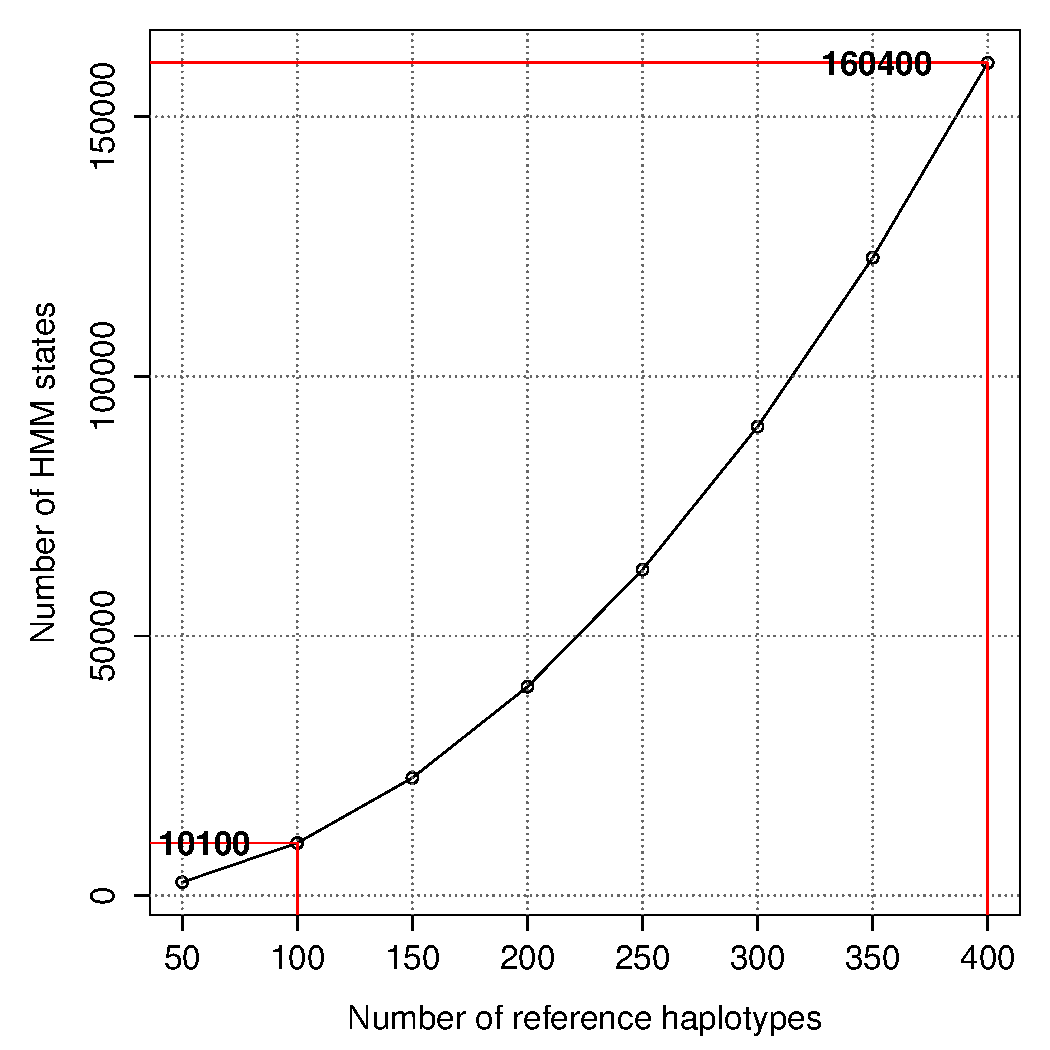
\includegraphics[width=\textwidth]{geneConv/figs/nStates}
    \end{center} 
    %\vspace{-20pt}
    \captionTitle{\textbf{Complexity of the gene conversion model.}}{
        The number of states is shown as a function of the total number of reference haplotypes.
        For a small number of haplotypes (50 in each reference population), there are 10,100 states.
        With 200 haplotypes in each population this increases to 160,400 states.
    \label{fig:GCnStates}} 
\end{figure}
\clearpage}

\paragraph*{Two-pass approach.}
To reduce the computation time for this model, we apply a two-pass approach.
In the first pass, we use only the crossover chain, and omit all gene conversion states from the model, reducing the number of states to ($n_1+n_2$).
The mutation parameters for both populations, which allow for a degree of copying error in the Markov chain, are set to approximately 0 (equivalent to machine epsilon).
This configuration forces the most likely state path (calculated using the Viterbi algorithm) to make a switch at each point a mismatch is detected between the copying haplotype and the unknown admixed haplotype (Figure \ref{fig:GCtwoPassSchematic}A).

Using this no-error Viterbi path, we identify long stretches (greater than 14 sites) where the admixed haplotype matches exactly to a reference haplotype.
These long stretches are likely to represent evolutionarily conserved shared haplotype segments.
Since our goal is to detect gene conversion events from one ancestral population against the background of the other population, these long stretches are unlikely to contain any information of interest (and this is supported by a lack of gene conversion events in our simulation).  
Instead, we look for regions where the Viterbi path makes short jumps between haplotypes of different reference populations, indicating a perfectly matching stretch of haplotype was not present in the reference.
These clusters of haplotype switches represent potential regions in which cross-population gene conversion events (or crossover) have disrupted linkage between neighboring sites.
We select haplotype stretches in the no-error Viterbi path that are short ($\le 14$ sites), and make a cross-population switch in haplotypes. % ([then back again?]).
For each of these stretches identified we select an additional 3 sites on each side of the stretch to capture events that may have occurred at the beginning or end.

We then make a second pass through the data, making a deeper inspection of the stretches of contiguous sites marked in the first pass though the data (Figure \ref{fig:GCtwoPassSchematic}B).
%Here the full HMM, with both crossover and gene conversion chains, is run only on only the sites that passed the criteria in the first pass.
Here the HMM is run using only the crossover chain (as in the first pass), except at sites marked for deeper inspection.
At these sites the gene conversion chain is turned on and we allow all possible transitions under the full HMM.
This technique allows a drastic reduction in the model complexity at sites that are unlikely to contain a gene conversion event (or at least those that are able to be detected by our model).
%%%
\afterpage{
\begin{figure}[P]
    \begin{center}
    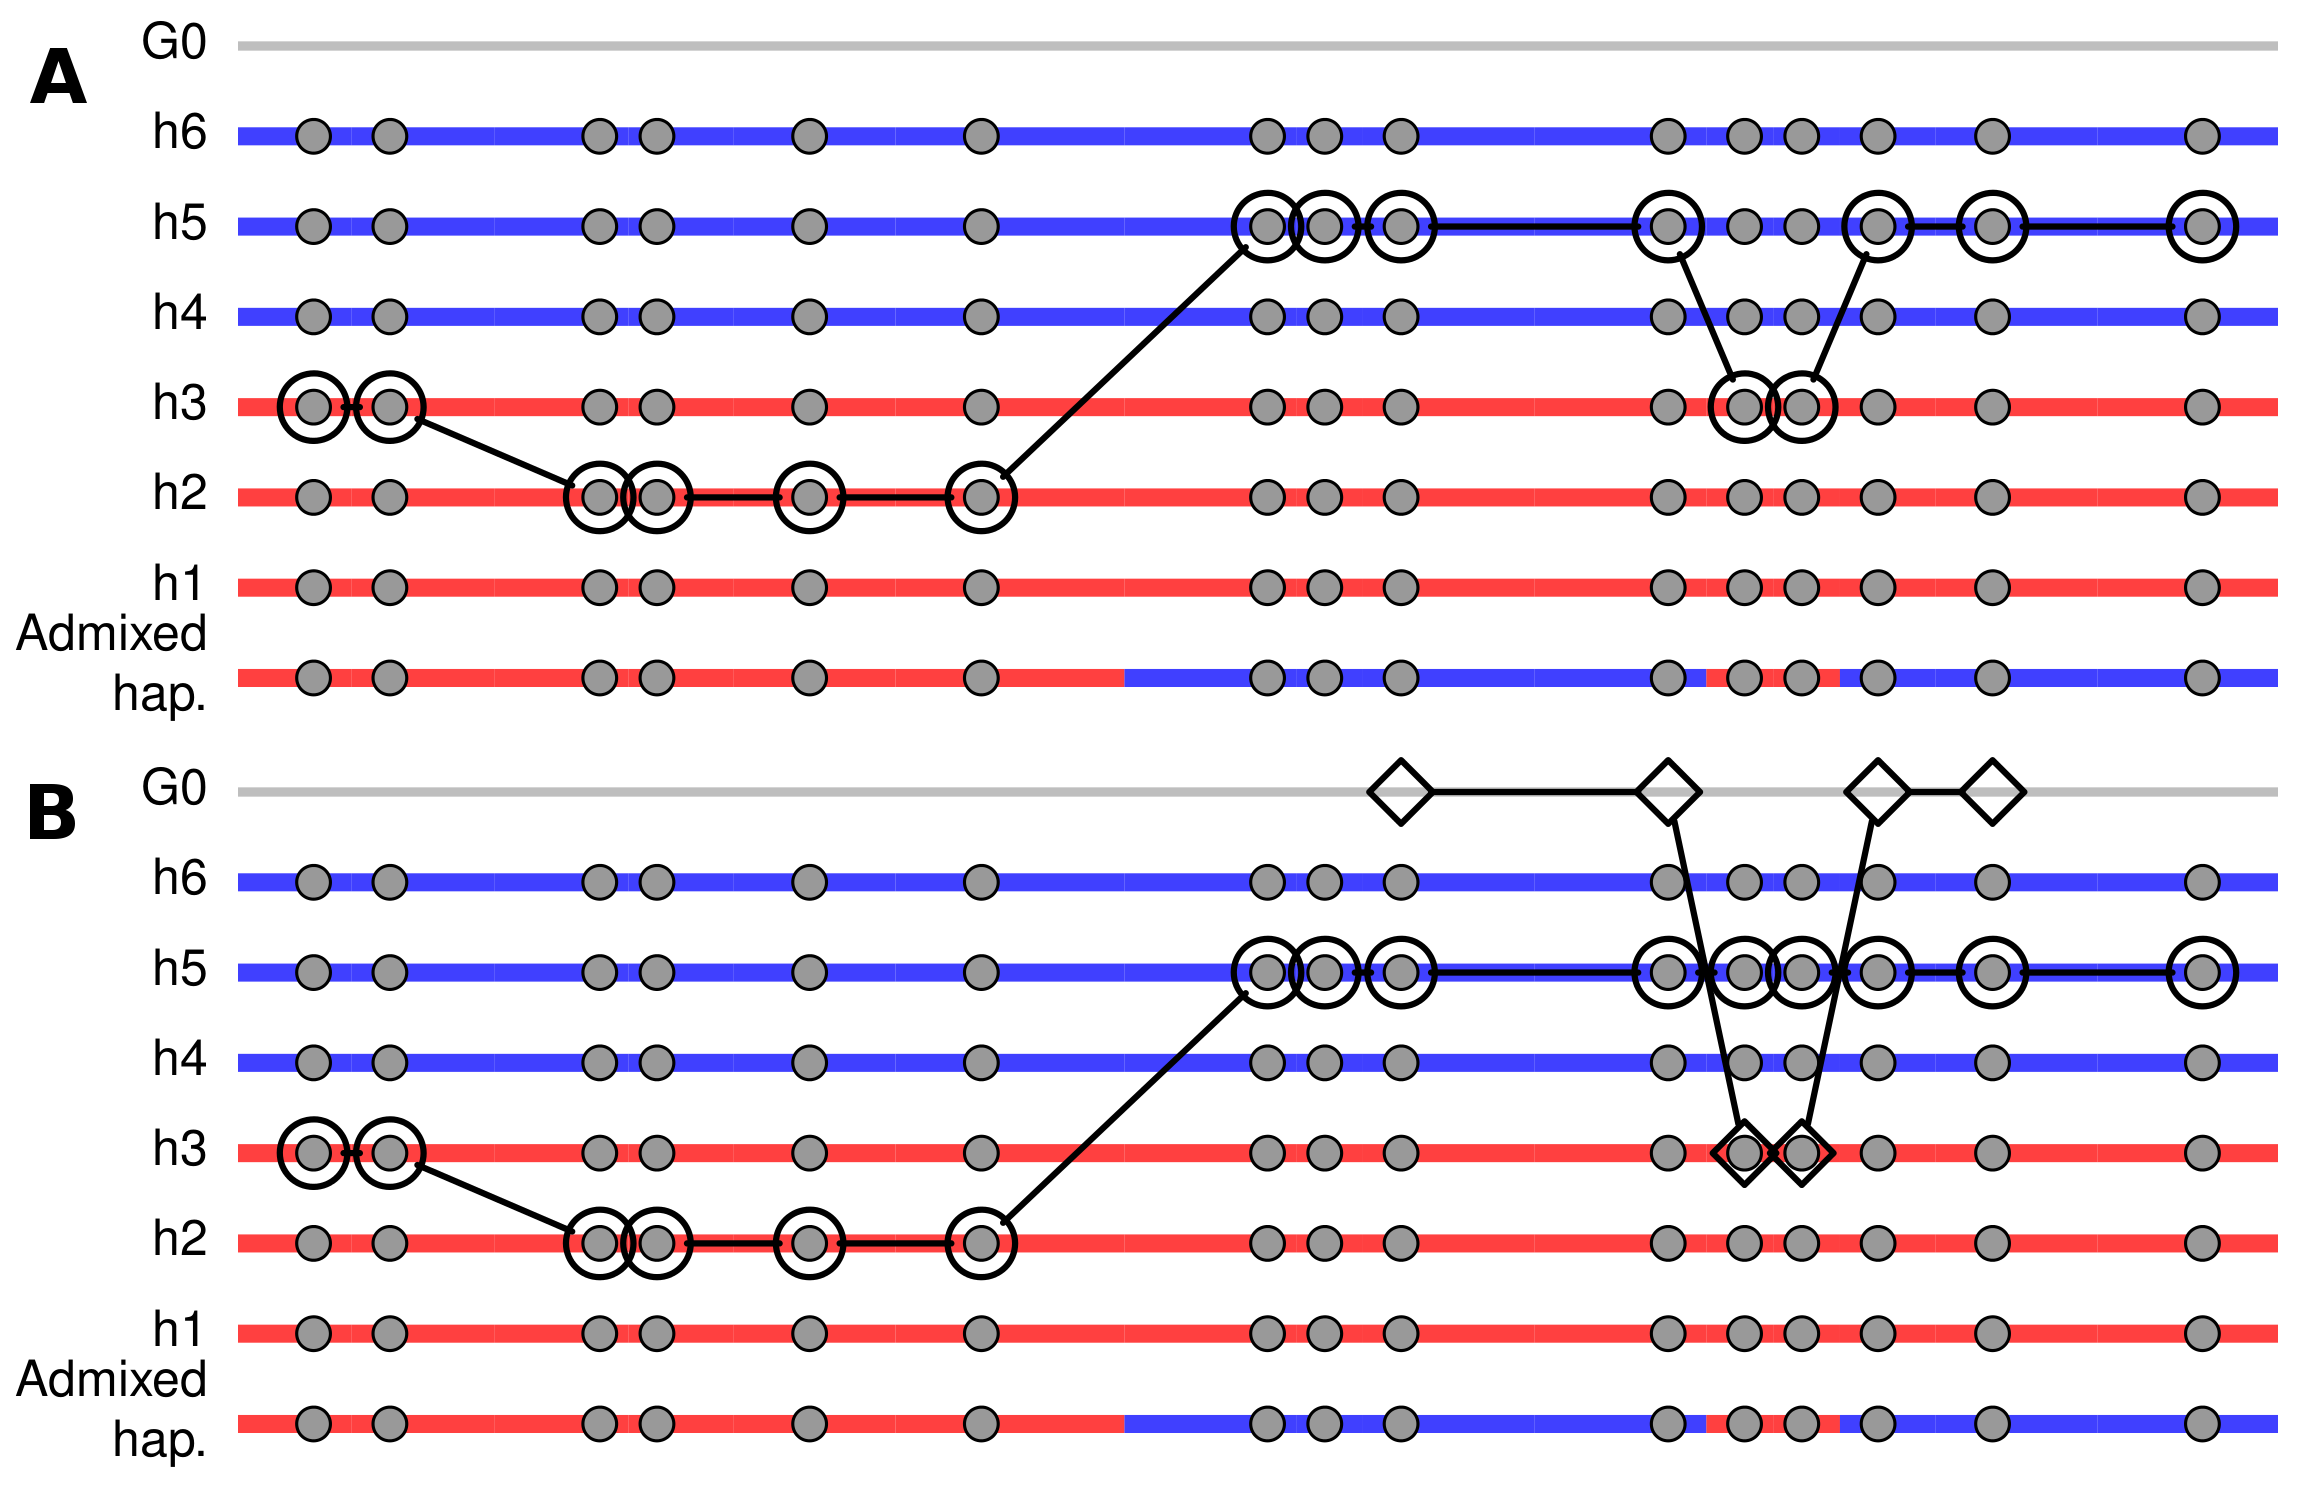
\includegraphics[width=\textwidth]{geneConv/figs/schematic_2pass.png}
    \end{center} 
    %\vspace{-20pt}
    \captionTitle{\textbf{Schematic of the two-pass HMM approach.}}{
        Each horizontal line is a haplotype, with blue and red colors designating segments that are representative of two divergent ancestral reference populations.
        Each column of circles represents the alleles of a SNP.
        The state path of haplotype transitions ($X$) is shown by open circles while the gene conversion state path ($G$) is shown in open diamonds.
        In \textbf{A} the gene conversion chain is not used and the crossover chain is forced to jump to $h3$ to accommodate the gene conversion.  
        In \textbf{B} the gene conversion chain is not used except for a few sites on either side of the putative gene conversion event.
    \label{fig:GCtwoPassSchematic}} 
\end{figure}
\clearpage}
%%%

Further reduction in computation time is achieved by running the second pass on smaller subsamples taken from the total body of reference haplotypes.
For example, with a group of 200 haplotypes in each reference population, we draw 10 random samples of 50 haplotypes from each.
We then run the reduced complexity model on the 10 subsets.
Finally, the results from each of the subsets are combined by taking the mean posterior probability of a cross-population gene conversion event.
This allows a drastic reduction in the number of total states, and thus a much faster run time.


\subsection{Simulation}
In order to test the ability of the model to identify gene conversion events, we first evaluate its performance using simulated data where the true GC events are known.
Data from the 1000 Genomes Project (Phase III\cite{1000G2015}) serves as source data from which we draw haplotypes for our parental populations.

Since our model attempts to infer recombination rates, the use of data 1000 Genomes data that was assembled and phased using a genetic map (the HapMap phase II map\cite{hapmap2007}) would introduce a potential bias.
In order to avoid this bias, we first re-phase the data.
We use SHAPEIT\cite{Delaneau2013} to construct phased haplotypes from genotype data.
SHAPEIT requires a genetic map as a prior input for phasing, so we create a map with the same intervals as the standard HapMap genetic map, but with the recombination rate at each interval set to 1.1 cM/Mb.
In addition, our method uses a genetic map, with estimates of the recombination rate at each site, to provide values for parameters for the per-generation crossover rate, $r$, and by extension, the gene conversion rate, $g$ (which is equal to $f r$).
As this also has the potential to introduce bias, we again use a genetic map with a fixed recombination rate.

To create simulated admixed haplotypes, we use a 1 Mb region on chr22, taking all phased haplotypes from two groups of reference populations.
For European haplotypes we select CEU, GWR, and TSI populations (n=399), and we select YRI and LWK for African populations (n=302).
We draw 100 haplotypes from each of two reference populations.
SNP density is thinned to keep 300 sites, and singleton variants are removed from the analysis.

An initial point admixture is then simulated for 50 haplotypes by drawing one haplotype from each reference population and creating a recombinant ``offspring'' haplotype.
The number of crossovers is determined by sampling from a Poisson distribution ($r = 1 / \mathrm{Mb}$).
Gene conversions are likewise placed under a Poisson process ($g = 10/1 \mathrm{Mb}$; $1/\lambda = 500 \mathrm{bp}$).
Following the initial admixture event, six subsequent generations were simulated using intra-population mating, with CO and GC events recorded each time they occurred. 
Our HMM is then run using the haplotypes from the simulated admixed population using the two-pass approach.

\subsection{Code availability.}
This C++ code for this model is available at \url{https://github.com/clcampbell/CGmix}.


%%%%%%%%%%%%%%%%%%%%%%%%%%%%%%%%%%%%%%%%
\section{Results}
%%%%%%%%%%%%%%%%%%%%%%%%%%%%%%%%%%%%%%%%


We test the performance of our model using simulated genomes on real human data from the 1000 Genomes Project\cite{1000G2015}.
Using a small sub-section of chromosome 22, we select parent haplotypes from CEU and YRI populations, representing individuals of European and African descent, respectively.
Recombination crossovers are placed with a rate of 1 / Mb, and gene conversions at 10 times this rate (10 / Mb).
We use a mixing proportion, $\mu$ = 0.5, instead of the 0.8 value estimated from previous methods\cite{Price2009}.
The location and type of each gene conversion is recorded for evaluation purposes.

Gene conversions can be classified into one of three types, based upon how our model will be able to detect them.
We are unable to detect GCs that do not overlap a SNP, and label these ``invisible'' GC events.
GCs that do overlap a heterozygous SNP, and do not produce any change in the alleles are labelled ``silent'' GC events.
Finally, GC events that overlap a SNP and produce a detectable change in the allele are termed ``non-silent'' events, and are the only ones that are detectable by our model.
Therefore, our results only account for non-silent gene conversion events, and we do not consider the other cases, even though they may occur as a result of the simulation.

For all GC events detected, we record the total posterior probability of finding a GC event at that site, and whether this is a real (non-silent) GC event.
Using a threshold of 0.5 for the posterior probability, we estimate the true positive rate at 8.0\%, while the false discovery rate is 27.3\%. % (Figure \ref{fig:GCperformance}).


% \afterpage{
% \begin{figure}[P]
% \begin{center}
%     %\includegraphics[width=\textwidth]{figs/TPR-FDR_NotUsingParentHaps.pdf}
%     \end{center} 
%     \vspace{-20pt}
%     \captionTitle{\textbf{Performance of the model.}}{
%     True positive (TPR) false discovery (FDR) rates from simulated data as a function of the threshold on posterior probability of a gene conversion event.
% \label{fig:GCperformance} }
% \end{figure}
% \clearpage}


\section{Discussion}

The detection of recombination within population genetic data using LD based approaches has been used in a number of studies in humans, yielding valuable results\cite{Mcvean2004,Myers2005,hapmap2007}.
A number of methods have been based on a model described by \citet{Li2003} in 2003, in which haplotypes are modeled as a mosaic of segments from other haplotypes.
Several extensions from this method have produced valuable models to detect gene conversion\cite{Gay2007}, and accurately infer admixture breakpoints\cite{Price2009,Hinch2011}.
The admixture approach to recombination is a promising one, especially considering the expanding availability of data on a number of human populations of diverse origins, many of them admixed.

The detection of gene conversion events has long been a difficult problem, owing to their small size, and the confounding effects of genotyping error.
Most studies focus on crossover and ignore the effects of gene conversion, which provides an incomplete picture of the recombination process as a whole.
In our model, the use of admixed genomes provides a unique leverage, in which we detect gene conversion events from one ancestral population against a contrasting background from the other.
In our model, we adopt the Li and Stephens model to include gene conversion, as in \citet{Gay2007}, and two reference populations, as in HAPMIX\cite{Price2009}.
This resulting model attempts to identify cross-population gene conversion events with a higher contrast.

The confounding effects of genotyping error and the small size of gene conversion events therefore constrain the sensitivity of the model substantially, which we report here to be 8\%.
This low sensitivity is expected, due to the nature of the problem, and this model can still be considered to be successful even when missing the vast majority of true events.
The detection of even a few hundred gene conversions in human data would represent a substantial advance in our knowledge.
The FDR of the model is far more important, and lowering this rate to under 10\% would be a key advance that would be necessary before the model can be run on admixed samples with any reliability.
Future work could focus on simplifying the model, and reducing the FDR.

% Simulation results show...

While the complexity of this model is quite high, we have made several advances that allow the computation time to be brought down.
First, we have reduced the state space by dividing the reference populations into ten random subsets.
The model was run on these subsets, and the results combined to generate an approximation to the model under the full set of reference haplotypes.
In addition, we built in the ability to run our model in two parts.
The first pass runs quickly, using only the crossover chain, and screens for potential breakpoints.
In the second pass, the full model with both CO and GC chains is used, but only on a subset of the sites that had been previously marked for deeper inspection.
These advances can potentially be generalized to other HMMs of similar structure in the future.
Despite these advances, the complexity is such that it is impractical to run this data on full genomes without significant advances in computing efficiency.
In addition inference using this model, while theoretically possible, is not practical.
Other models use maximum likelihood methods to estimate optimal parameter settings.
For example, in the Li and Stephens model, this technique was used to estimate $\hat{\rho}$ from human data, providing approximations to the recombination rate across the genome.

This model provides a method to detect recombination and gene conversion in admixed population genetic data.
While the complexity of this model is high, it has the potential to be used in human data, especially as the availability of admixed data increases.
Combined with an increase in computing efficiency, or a redesign of the model, this admixture approach has promise for future work to further characterize gene conversion in the human genome.
% Future work to identify gene conversion events from population genetic data could focus on admixed genomes.




%%%%%%%%%%%%%%%%%%%%%%%%%%%%%%%%%%%%%%%%
%%%%%%%%%%%%%%%%%%%%%%%%%%%%%%%%%%%%%%%%
\clearpage
\renewcommand{\bibname}{References}
\bibliographystyle{ccampbell_thesis}
\begingroup
    \setlength{\bibsep}{10pt}
    \linespread{1}\selectfont
    \bibliography{/home/ccampbell/Dropbox/papers/recombination,/home/ccampbell/Dropbox/papers/thesis,/home/ccampbell/Dropbox/papers/GeneConversion}
\endgroup
%%%%%%%%%%%%%%%%%%%%%%%%%%%%%%%%%%%%%%%%
%%%%%%%%%%%%%%%%%%%%%%%%%%%%%%%%%%%%%%%%

